\documentclass[11pt] {article}
\usepackage{graphicx}

\begin{document}

$$
\includegraphics[scale = 4]{alatoo}$$

\vspace{5mm} %5mm vertical space
\begin{center}
PART 4

ELECTRICITY AND  MAGNETISM         
                 
Electric Fields 

Gauss’s Law

Electric Potential

Capacitance and Dielectrics

Current and Resistance

Direct-Current Circuits

Magnetic Fields

Sources of the Magnetic Field

Faraday’s Law

Inductance

Alternating-Current Circuits

Electromagnetic Waves

\end{center}
\vspace{5mm} %5mm vertical space
\hfill Name: S.Betul Polat

\hfill Course Name: Physics

\hfill Group: COM-18

\vspace{25mm} %5mm vertical space
							$$ACKNOWLEDGEMENT$$

First of all I would like to thank our lecturer Tahir Aslan for supporting  us in learning the Physics and for supporting us when we need help.

Beside from my lecturer, I like to thank my other students for their effort.

Completing their report and for carrying the spirit of solidarity.

We, the students, believe that we will be successful citizens and educators if we receive the necessary education to guarantee our future.

In order to accomplish some things, it is necessary to work hard and make efforts. 

We need an environment where we can work hard to survive the challenges and go on new and bright days, and we need supporters who trust us. 

But success starts with self-confidence, so first of all thanks to our family and friends and of course our teachers.


\vspace{25mm} %5mm vertical space

							$$INTRODUCTION$$

In this universe we live in, there are structures of things around us and many science-based formations we cannot see.

For example, I would like to talk briefly about Physics, such as electricity, light, sound, magnetic formations, and most importantly, 

the structure and formations of atoms. We have a lot to learn from physics in our lives.

The rules of physics have a great place in our normal life. 

Weight, gravity, force, distance, speed, height, electronic light, and so on, these are part of physics, 

and a lot of inventions about them are also available on the internet.

\vspace{30mm} %5mm vertical space
--------------------------------------------------------------------------------------------

p a r t 4 - Electricity and Magnetism

Electric Fields
\begin{center}
Charging Objects by Induction
\end{center}
There are many ways to charge an object in Physics, one of these methods is called as induction.

The situation is as follows, the charged object is brought next to the neutral conductor, but that conductor is not touched.

Electrical conductors are materials in which some of the electrons are free electrons that are not bound to atoms and can move relatively freely through the material; 

electrical insulators are materials in which all electrons are bound to atoms and cannot move freely through the material.

$$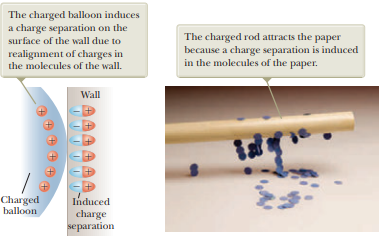
\includegraphics[scale = 0.7]{img1}$$

--------------------------------------------------------------------------------------------

Coulomb’s Law
\begin{center}
The coulombs are briefly expressed as the magnitude of the electrostatic attraction or thrust force between the two points is directly proportional to the magnitude of the charges and inversely proportional to the square of the distance between them.

From experimental observations, they find that the magnitude of the electric force (sometimes called the Coulomb force) between two point charges is given by Coulomb’s law.

$$Fe = \frac{ke |q1||q2|} {r^2}$$

$$ke =  8.987 6 x 10^9 N .  m2/C2$$

$$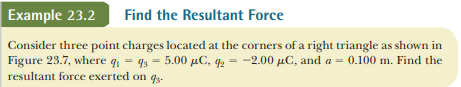
\includegraphics[scale = 1]{img2}$$

$$F = ke \frac {|q1||q2|} {a^2}$$

$$= F_13 = \frac{8,9 x 10^9 . 25 x 10^-1} {\sqrt{2}x 10^-1^2} = 11,125N . r_12$$
\end{center}

\vspace{10mm} %5mm vertical space
--------------------------------------------------------------------------------------------

Gauss’s Law
\begin{center}
Electric Flux
\end{center}
From the SI units of E and A, we see that FE has units of newton meters squared per coulomb (N . m2/C). Electric flux is proportional to the number of electric field lines penetrating some surface.

If the surface under consideration is not perpendicular to the field, the flux through it must be less than that given by

$$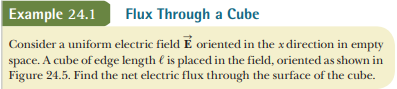
\includegraphics[scale = 1]{img3}$$

$$Fe = El^2 . cos180 = -El^2$$

$$F_e2 = El^2 . cos0 = El^2$$

$$Fe1 + Fe_2 = El^2 - El^2 = 0$$

\begin{center}
--------------------------------------------------------------------------------------------
\end{center}
chapter 25 - Electric Potential
\begin{center}
Electric Potential and Potential Difference
\end{center}

When a charge q is placed in an electric field E created by some source charge distribution, the particle in a field model tells us that there is an electric force q E acting on the charge. 

This force is conservative because the force between charges described by Coulomb’s law is conservative. 

If the charge is free to move, it will do so in response to the electric force. 

Therefore, the electric field will be doing work on the charge. 

This work is internal to the system. 

This situation is similar to that in a gravitational system: When an object is released near the surface of the Earth, the gravitational force does work on the object.

Change in potential energy is :  

$$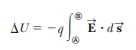
\includegraphics[scale = 1]{ing5}$$

electric potential is :

$$V =\frac{U} {q}$$

Because electric potential is a measure of potential energy per unit charge, the SI unit of both electric potential and potential difference is joules per coulomb, which is defined as a volt (V):

$$1V = \frac{1J} {C}$$


--------------------------------------------------------------------------------------------
\begin{center}
Potential Difference in a Uniform Electric Field
\end{center}

The formula for calculating the electric potential difference is:

V = Ed, V is expressed as volts, that is the potential difference and E is the electric field
\vspace{10mm} %5mm vertical space
$$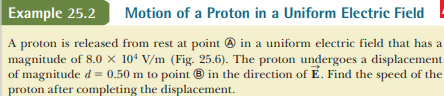
\includegraphics[scale = 1]{img6}$$

$$E = 8 x 10^4 V/m$$
$$\frac{1}{2 mv^2} = qV$$
$$Ki + Ui = K_f + U_f$$
$$0 + qV_i = \frac{1}{2mV_f^2 + qV_f}$$
$$V = \sqrt{2gV/m} $$
\vspace{20mm} %5mm vertical space
$$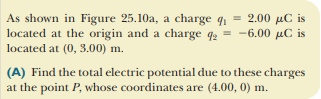
\includegraphics[scale = 1]{img7}$$

$$V_p = k_e(\frac{q_1}{q_2} + \frac{q_2}{r_2})$$

$$V_p = (8.988 x 10^9 N . m^2/C^2)(\frac{2.00 x 10^-6 C} {4.00m} + \frac{-6.00 x 10^-6C} {5.00m} = -6.29 x 10^3V)$$

\vspace{20mm} %5mm vertical space
--------------------------------------------------------------------------------------------
\begin{center}
c h a p t e r 26 -  Capacitance and Dielectrics
\end{center}
The capacitance C of a capacitor is defined as the ratio of the magnitude of the charge

on either conductor to the magnitude of the potential difference between the conductors:

\begin{center}
Calculating Capacitance
\end{center}
$$C = \frac{Q}{\Delta{V}}, V = V_b - V_a$$

$$K_e = \frac{1}{4} {\pi{E_0}}$$

\vspace{25mm} %5mm vertical space
$$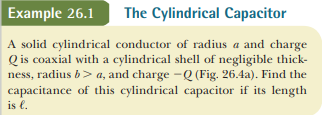
\includegraphics[scale = 1]{img8}$$

$$E . A = \frac{Q}{E_0}$$

$$E . 2\pi{rl.E_0} = \frac{l}{2\pi{rlE_0}} =  \frac{l}{2k_eln(b/a)}$$

\vspace{35mm} %5mm vertical space
--------------------------------------------------------------------------------------------
\begin{center}
Combinations of Capacitors
\end{center}

When capacitors are connected in series, the magnitude of charge Q on each capacitor is same. 

The potential difference across C1 and C2 is different i.e., V1 and V2. 

The ratio Q/V is called as the equivalent capacitance C between point a and b.

$$C = \frac{Q}{\Delta{V}} = Q = CV$$

$$Ceq = ?$$

$$\Delta{V} = \Delta{V_1} = \Delta{V_2}$$

$$Ceq = \frac{C_1 . \Delta{V} + c_2 \Delta{V_2}}{\Delta{V}}$$

$$Ceq = C_1 + C_2$$

\vspace{10mm} %5mm vertical space
$$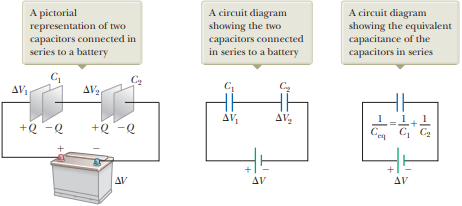
\includegraphics[scale = 1]{img10}$$

\vspace{5mm} %5mm vertical space
$$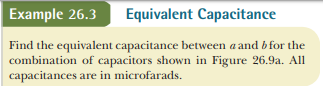
\includegraphics[scale = 1]{img11}$$

$$\frac{1}{C_eq} = \frac{1}{C_1} + \frac{1}{C_2} = \frac{1}{4.0} + \frac{1}{4.0}$$
$$C_eq = 2.0$$

\begin{center}
--------------------------------------------------------------------------------------------
\end{center}
chapter- 27 Current and Resistance
\begin{center}
 Electric Current
\end{center}
Electric current is a flow of electrons or electric charge in a given circuit and carried negative or positive charged electrons.

$$I_avg = \frac{\Delta{Q}}{\Delta{t}} , I = \frac{dq}{dt}$$

$$V = \delta{I}{R}$$

$$1A = 1 C/ s$$

$$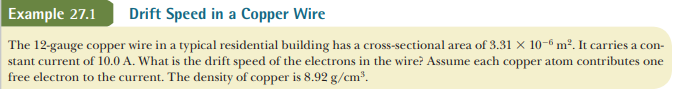
\includegraphics[scale = 0.8]{img12}$$

$$I = n . A . V_1 . q$$

$$V_d = \frac {I}{n.Aq} =$$

$$n = \frac{N_A}{V} = 6 x 10^23$$
$$V_d = 2.23 x 10^-4 m/s$$

--------------------------------------------------------------------------------------------
\begin{center}
27.2 Resistance
\end{center}
It helps us to measure the current flow in an electrical circuit. Resistance is measured in ohms.

$$R = \frac{V}{I}$$

$$\Delta{V} = El$$

$${1}\Omega = 1V/A$$

$$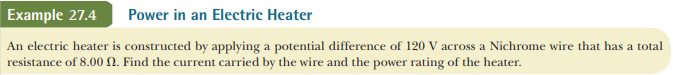
\includegraphics[scale = 0.8]{img13}$$

$$I = \frac{\Delta{V}}{R} = $$

$$\frac{120V}{{8.00}\Omega} = 15.0 A$$

$$P = I^2 R = (15.0A)^2({8.00}\Omega) = 1.80kW$$

--------------------------------------------------------------------------------------------

c h a p t e r - 28 Direct-Current Circuits
\begin{center}
28.1 Electromotive Force
\end{center}
ElectroMotive force can be described as 'emf' or 'E' means energy per unit, its can be electric generator or a battery

The emf e of a battery is the maximum possible voltage the battery can provide between its terminals.
$${\Delta{V}} = IR = E - Ir$$
$$E = I(R+r)$$
$$I = \frac{E}{R+r}$$
$$P = I . \Delta{V}$$
$$P = I^2(R + r)$$

--------------------------------------------------------------------------------------------

$$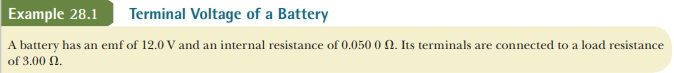
\includegraphics[scale = 0.8]{img14}$$

$$I = \frac{E}{R+ r} = \frac{12.0V}{{3}\Omega + {0.05}\Omega} = 3.95A$$

$$\Delta{V} = E - Ir = 12.0V - (3.93A)({0.05}\Omega) = 11.8V$$

--------------------------------------------------------------------------------------------

28.2 Resistors in Series and Parallel 

$$I = I_1 = I_2$$

Resistors in series:

$$R_eq = R_1 + R_2 + R_3 + ....$$

$$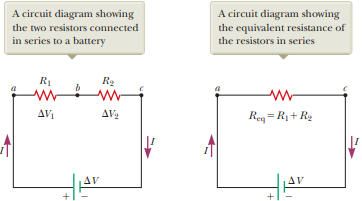
\includegraphics[scale = 0.8]{img15}$$

Resistors in parallel:

$$R_eq = \frac{1}{R_1} + \frac{1}{R_2} + \frac{1}{R_3} + ...$$

$$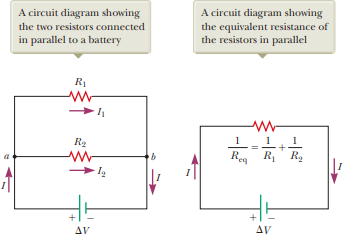
\includegraphics[scale = 0.8]{img16}$$

$$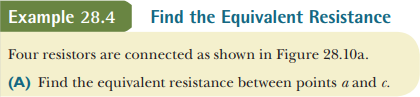
\includegraphics[scale = 0.8]{img17}$$

$$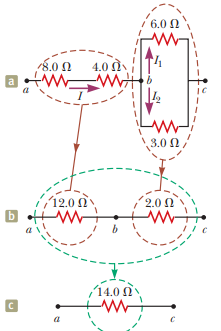
\includegraphics[scale = 0.8]{img18}$$

$$R_eq = {8}\Omega + {4}\Omega = {12}\Omega$$

$$\frac{1}{R_eq} = \frac{1}{{6}\Omega} + \frac{1}{{3}\Omega} = \frac{3}{{6}\Omega} = {2}\Omega$$
$$R_eq = {12}\Omega + {2}\Omega = {14}\Omega$$


\end{document}